\documentclass[paper=a4, fontsize=11pt]{scrartcl} % A4 paper and 11pt font size

\usepackage[T1]{fontenc} % Use 8-bit encoding that has 256 glyphs
\usepackage{fourier} % Use the Adobe Utopia font for the document - comment this line to return to the LaTeX default
\usepackage[english]{babel} % English language/hyphenation
\usepackage{amsmath,amsfonts,amsthm,amssymb} % Math packages

\usepackage{algorithm, algorithmic}
\renewcommand{\algorithmicrequire}{\textbf{Input:}} %Use Input in the format of Algorithm  
\renewcommand{\algorithmicensure}{\textbf{Output:}} %UseOutput in the format of Algorithm  

\usepackage{graphicx}
\usepackage{blindtext}
\usepackage{enumerate}
\usepackage{ulem} 
\usepackage{pdfpages}

\usepackage{listings}
\lstset{language=Matlab}

\usepackage{lipsum} % Used for inserting dummy 'Lorem ipsum' text into the template

\usepackage{sectsty} % Allows customizing section commands
\allsectionsfont{\centering \normalfont\scshape} % Make all sections centered, the default font and small caps

\usepackage{fancyhdr} % Custom headers and footers
\pagestyle{fancyplain} % Makes all pages in the document conform to the custom headers and footers
\fancyhead{} % No page header - if you want one, create it in the same way as the footers below
\fancyfoot[L]{} % Empty left footer
\fancyfoot[C]{} % Empty center footer
\fancyfoot[R]{\thepage} % Page numbering for right footer
\renewcommand{\headrulewidth}{0pt} % Remove header underlines
\renewcommand{\footrulewidth}{0pt} % Remove footer underlines
\setlength{\headheight}{13.6pt} % Customize the height of the header

\numberwithin{equation}{section} % Number equations within sections (i.e. 1.1, 1.2, 2.1, 2.2 instead of 1, 2, 3, 4)
\numberwithin{figure}{section} % Number figures within sections (i.e. 1.1, 1.2, 2.1, 2.2 instead of 1, 2, 3, 4)
\numberwithin{table}{section} % Number tables within sections (i.e. 1.1, 1.2, 2.1, 2.2 instead of 1, 2, 3, 4)

\setlength\parindent{0pt} % Removes all indentation from paragraphs - comment this line for an assignment with lots of text

\newcommand{\horrule}[1]{\rule{\linewidth}{#1}} % Create horizontal rule command with 1 argument of height
\newcommand*{\dif}{\mathop{}\!\mathrm{d}}

\title{	
\normalfont \normalsize 
\textsc{Shanghai Jiao Tong University, UM-SJTU JOINT INSTITUTE} \\ [25pt] % Your university, school and/or department name(s)
\horrule{0.5pt} \\[0.4cm] % Thin top horizontal rule
\huge Technical Communication\\ HW3 \\ % The assignment title
\horrule{2pt} \\[0.5cm] % Thick bottom horizontal rule
}

\author{Yu Cang \quad 018370210001} % Your name

\date{\normalsize \today} % Today's date or a custom date

\begin{document}

\maketitle % Print the title

\section{Mind Map}
	\begin{figure}[!h]
		\centering
		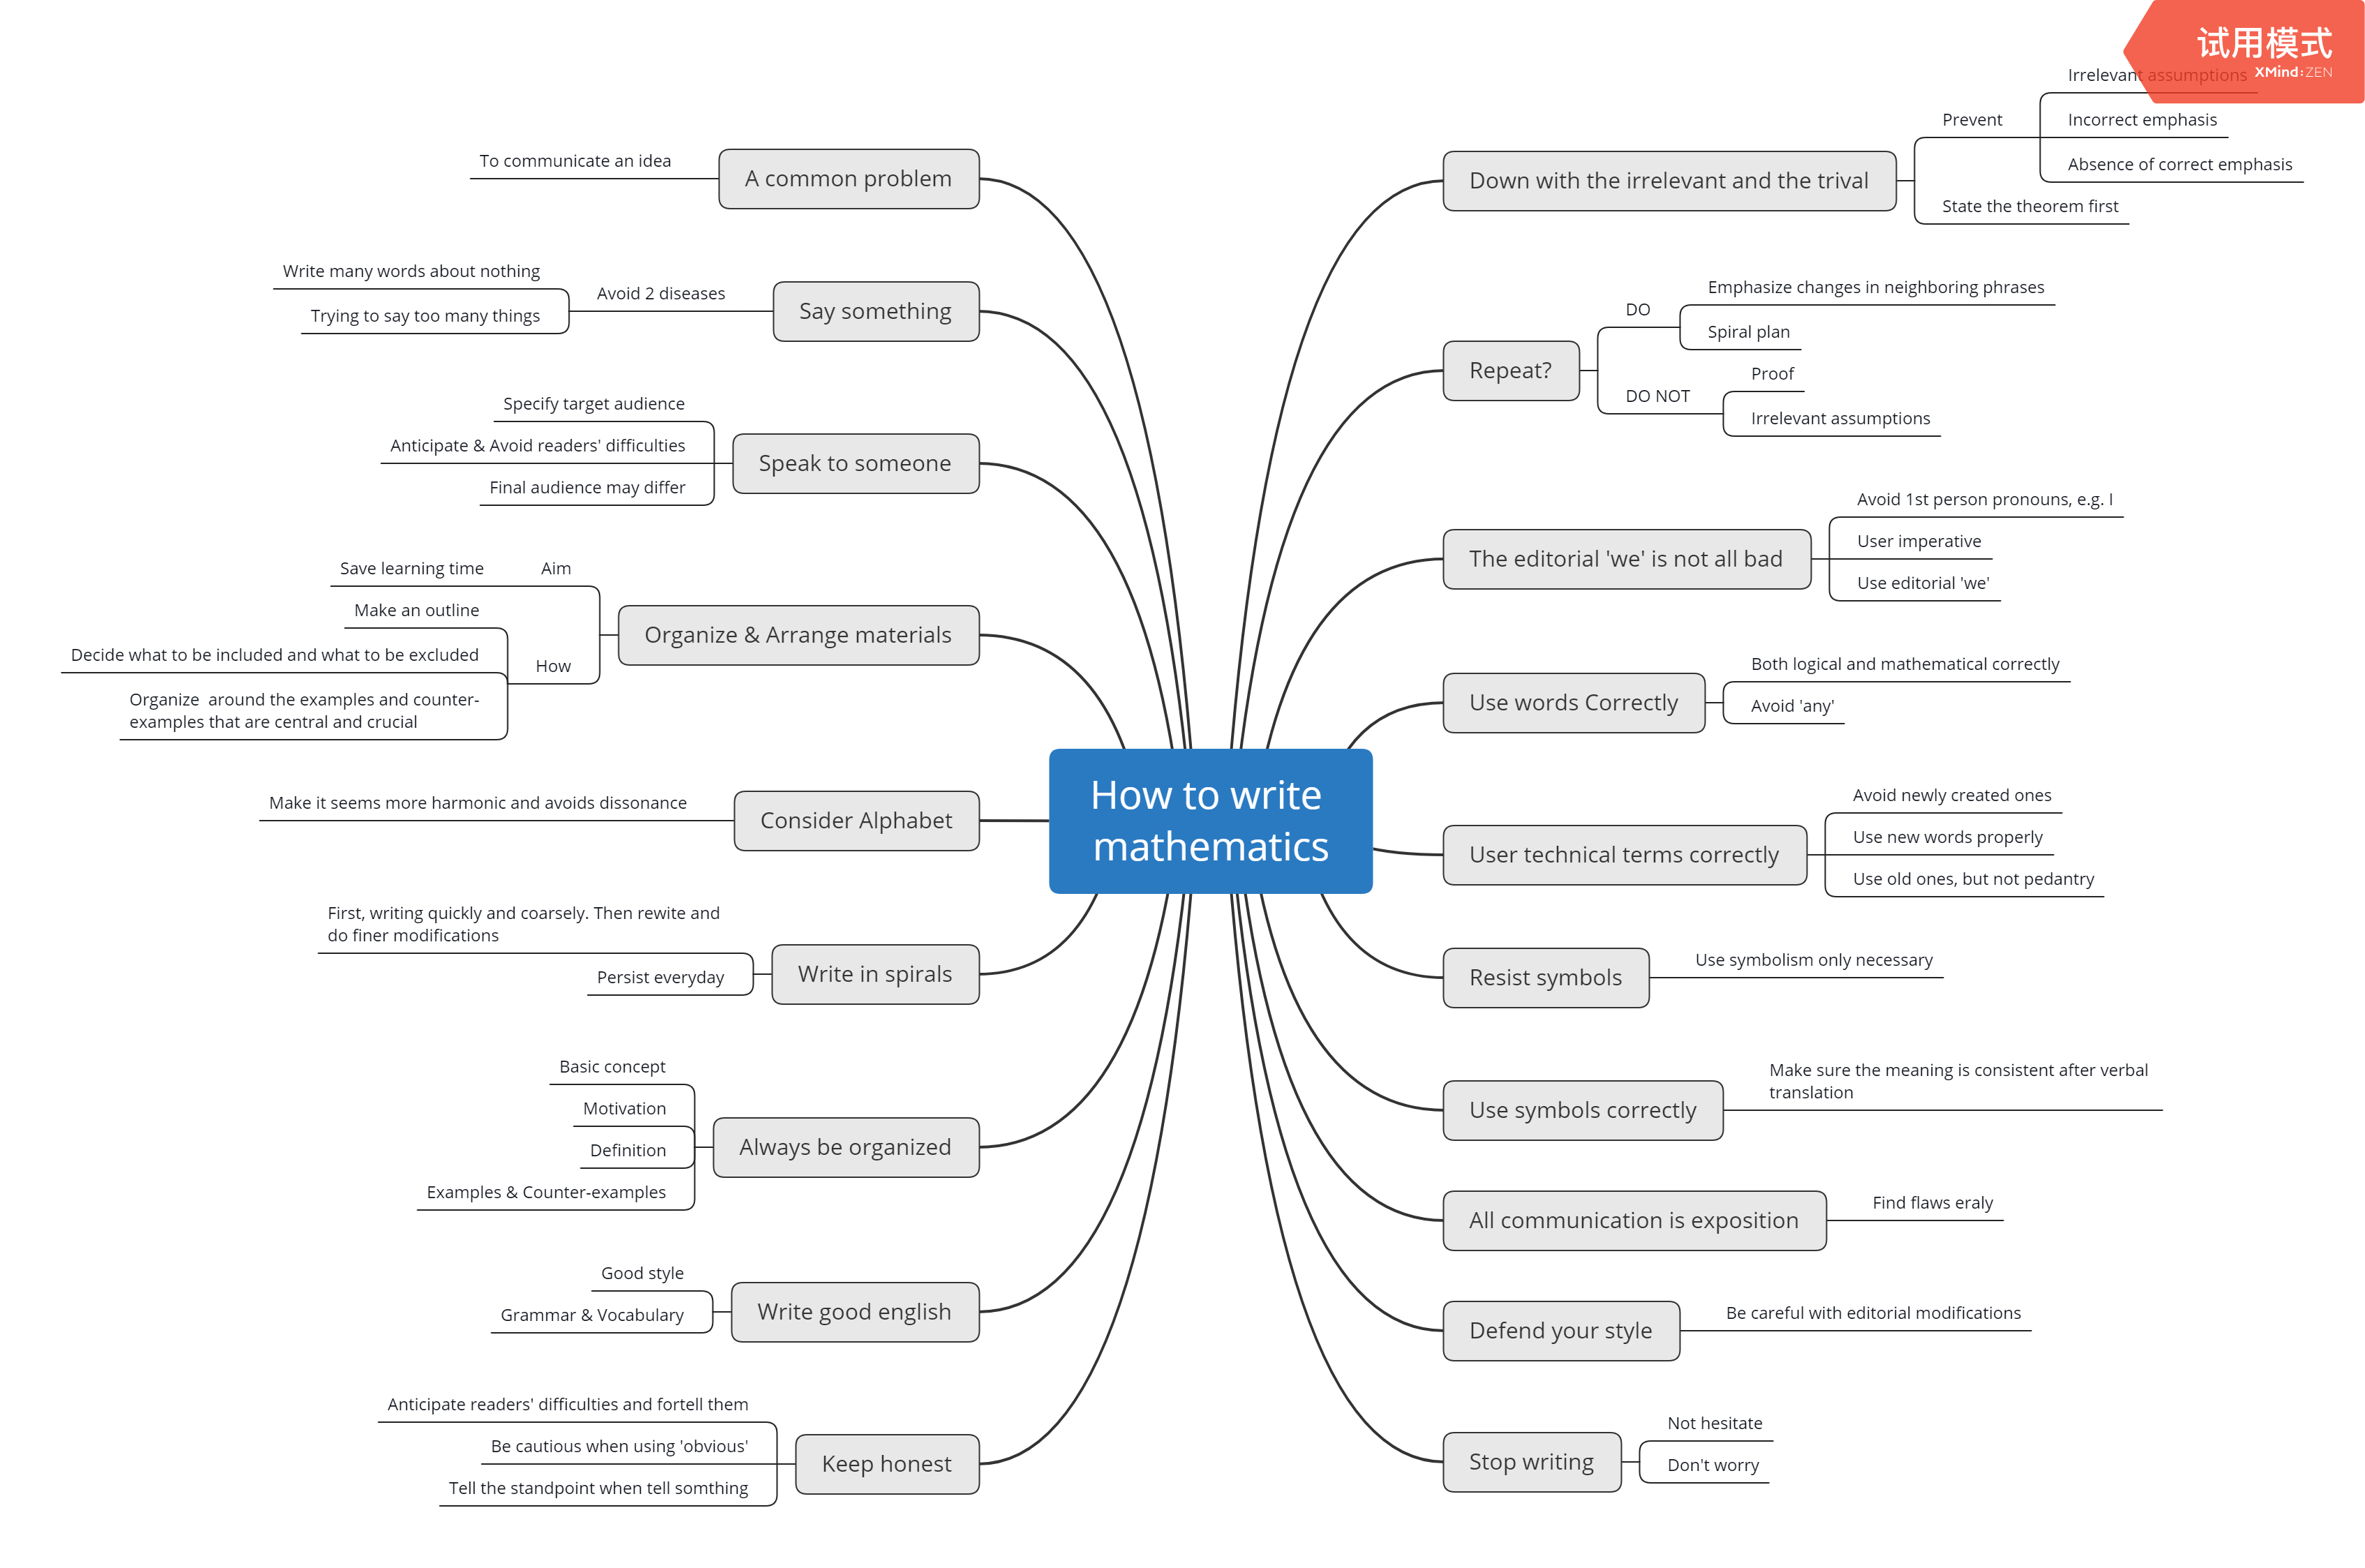
\includegraphics[scale=0.11]{pic/mind_map.png}
		\caption{How to write mathematics}
		\label{fig:htwm}
	\end{figure}


\section{Group Exercise}
	After discussion, we all think figures are generally properly used in this article, and comments from us are listed as below.
	
	\subsection{Comments from Yu Cang}
		From my point of view, most of the pictures used are of high quality and are both clear and concise. Most of the sketches are showed in 2D mode, which avoid 3D distortion and are easy to identify their meanings. Combination of colors are well arranged, where contrast is apparent and is suitable for printing and visualization. Line plots like Fig. 7 and Fig. 8 are simple and clear, without too many curves exhibited in one plot, distinctions and trends are well reflected. Besides, one remarkable point is that all the labels, if necessary, are accompanied with precisely stated units, which facilitates readers when making comparison and judgement. \newline 

		However, some details in these figures need to be furnished. The arrows in Fig. 5 are too dense. The ending points of indicating lines in Fig. 9 seems randomly placed, without a consistent compliance. Further, the gray figure in Fig. 10 may not reveal the distinctions well enough, and may get blurred when printed in black and white.
		
	\subsection{Comments from Ronghan Chen}
		Generally, the figures in the article look clear at the first sight. The sketches are beautiful. But if we look carefully, we can find many flaws. First, the tips of the arrows are not consistent. For fig. 1, the gap between arrows and targets are different. For fig. 5, the arrows on the right lie on the edges of targets, while the arrow on the top sticks into the target. Second, some of the labels are bad. For fig. 6, fig. 7 and fig. 9, the labels of the axis are a bit vague compared to fig. 10. Third, some texts on the figures are hard to read. For fig. 4, the direction of the words should keep horizontal. For fig. 3, the serial numbers are hard to see. Fourth, the selection of thickness is bad. The arrows in fig. 9 are too thick, as well as the line in fig. 11. In my point of view, I think fig. 8 is the best one of all the figures.
	
	\subsection{Comments from Rui Gao}
		The figures in the paper by Johnson and Popil are of acceptable quality but not the best among what I have seen. The choice of color are well designed to facilitate reading. The size of words within the figures are designed to be slightly larger than the size of the text. The information within each figure is clearly conveyed. I could have a coarse idea of the whole topic after reading these figures only (i.e. they speak for themselves).\newline
		
		However, I could see that the figures blur slightly even at 100\% size, which means that when printed on A4 paper (equal to 120\% size) they would also blur. This also indicate that the figures are not vector plots, and the dpi is not high enough. In addition, while the arrows are large and clear enough, the endings are not unified (there are arrows that ends before, at, and after the object they are indicating, for example in figure 1). While the font size is well designed, the fonts in different figures seems to be different (switching between bold and normal). The colorbars in Fig. 10 are not aligned with each other in an unnecessary manner. A few figures seems to be stretched slightly, like Fig. 6.
		
			
\section{Writting skills}
	\begin{enumerate}
		\item 
			``\textbf{Just act naturally}'': `naturally' is not suitable to be adverb for `act'.\newline
			``\textbf{Please give your unbiased opinion}'': No objective in this sentence.\newline
			``\textbf{I need an exact estimate by Friday}'': The two words: `exact' and `estimate' contradict with each other.

		\item 
			Before the agent was \sout{completely} able to \sout{finish} explain\sout{ing} the \sout{various} differences between \sout{all of} the \sout{many} outdoor event packages her company was offering, the customer changed his \sout{future} plans.
	\end{enumerate}

\section{\LaTeX}
	Listed as follows
	\includepdf[pages=2]{assignment.pdf}

\end{document}